\begin{center}
   \textbf{\titlePageWorkType~№\titlePageWorkNumber~\titlePageWorkPart}
\end{center}

\textbf{Тема}: <<\titlePageTopic>>

\textbf{Цель работы}: 

\begin{enumerate}
   \item Знакомство со структурой файла листинга, получаемого при ассемблировании, структурой машинных команд процессора.
   \item Изучение основных приемов отладки программ и основных возможностей отладчика Turbo Debugger (TD).
\end{enumerate}

\begin{center}
   \textbf{Ход работы}:
\end{center}



\subparagraph{Задание 4.1}

\textbf{Условие}:
\begin{itemize}
   \item Изучить предложенный материал по структуре и назначению полей файла листинга ассемблерной программы. 
   \item Изучить структуру машинной команды.
\end{itemize}

\textbf{Решение}:

\begin{table}[!ht]
   \centering
   \caption{Структура листинга}
   \begin{tabular}{|l|p{1.3cm}|l|p{2cm}|l|l|} 
      \hline
               & 11           & 0003      & 8E D8        & Metka1:   mov   ds, ax   ; установить регистр DS \\ \hline
      глубина  & номер строки & смещение  & машинный код & исходный текст программы                         \\ \hline
   \end{tabular}
\end{table}



\subparagraph{Задание 4.2}

\textbf{Условие}:
Пользуясь информацией лаб.раб.1, написать программу \path{Lab2.asm}, работающую по следующему алгоритму:
\begin{itemize}
   \item вывести на экран первые N символов фамилии студента (использовать функцию 40h DOS INT 21h) – число N задается преподавателем;
   \item вывести строку полностью в цикле N-1 раз на экран. Привести программу в отчете.
\end{itemize}

\textbf{Решение}:

\lstinputlisting[
   name=Lab2.asm,
   language={[x86masm]Assembler},
   tabsize=8,
   basicstyle=\ttfamily\scriptsize,
   numbers=left,
]
{../../src/lab2.asm}

\newpage

\begin{lstlisting}[language=Terminal]
$ C:\tasm\tasm.exe Lab2.asm
\end{lstlisting}
   
\begin{lstlisting}[language=Out]
Turbo Assembler  Version 2.0  Copyright (c) 1988, 1990 Borland International

Assembling file:     Lab2.asm
Error messages:      None
Warning messages:    None
Passes:              1
Remaining memory:    475k
\end{lstlisting}

\begin{lstlisting}[language=Terminal]
$ C:\tasm\tlink.exe LAB2.OBJ
\end{lstlisting}

\begin{lstlisting}[language=Out]
Turbo Link  Version 2.0  Copyright (c) 1987, 1989 Borland International
\end{lstlisting}

\begin{lstlisting}[language=Terminal]
$ LAB2.EXE
\end{lstlisting}

\begin{lstlisting}[language=Out]
Galan
Galanin
Galanin
Galanin
Galanin
\end{lstlisting}



\subparagraph{Задание 4.3}

\textbf{Условие}:
Получить файл листинга и внимательно ознакомиться с его форматом и содержимым.

\textbf{Решение}:

\begin{lstlisting}[language=Terminal]
$ C:\tasm\tasm.exe /l Lab2.asm
\end{lstlisting}

\begin{lstlisting}[language=Out]
Turbo Assembler  Version 2.0  Copyright (c) 1988, 1990 Borland International

Assembling file:   Lab2.asm
Error messages:    None
Warning messages:  None
Passes:            1
Remaining memory:  469k
\end{lstlisting}

Создался объктный файл LAB2.OBJ и файл листинга LAB2.LST.

\begin{figure}[h]
    \centering
    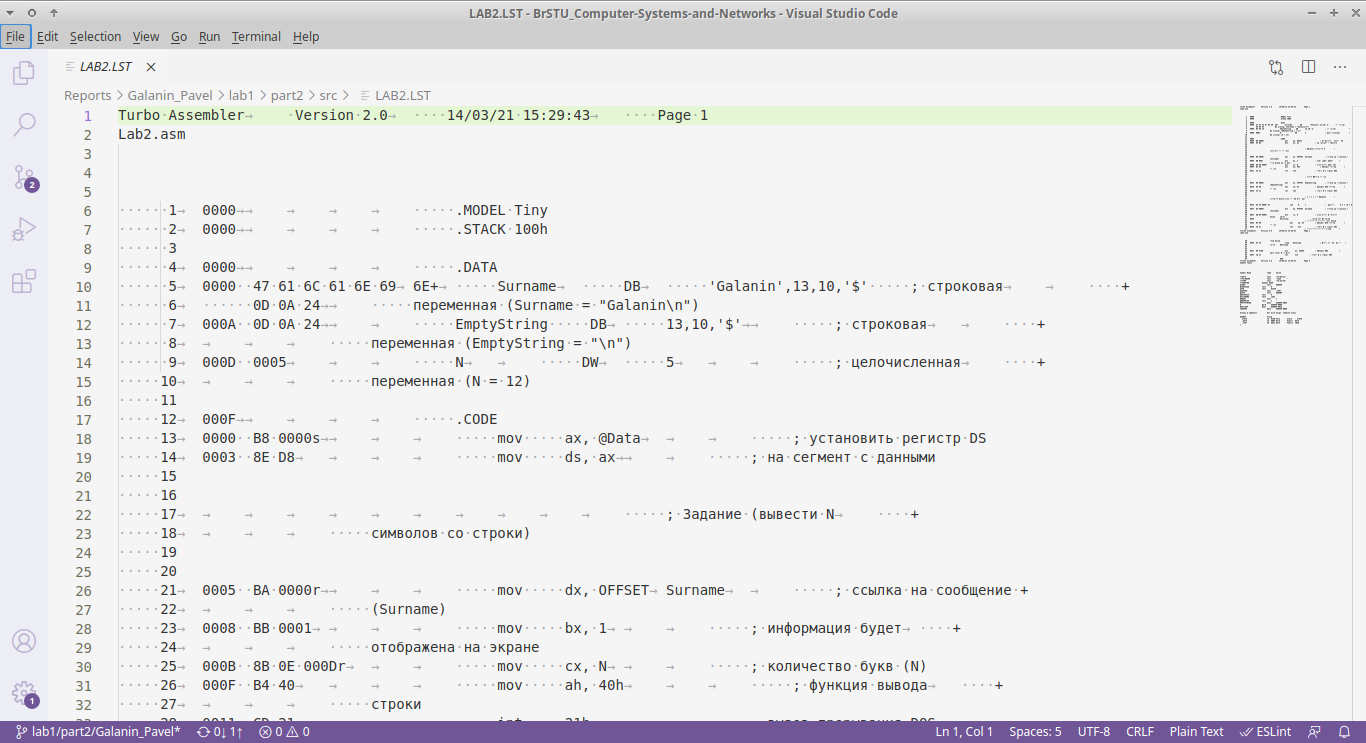
\includegraphics[width=18cm]{../_INCLUDES/lst.png}
    \caption{LAB2.LST в VS Code}
\end{figure}



\subparagraph{Задание 4.4}

\textbf{Условие}:
В любой инструкции с двумя операндами удалить один операнд и проассемблировать программу с получением файла листинга. Какие выходные файлы создаются в этом случае? Что добавляется в листинге? Привести результаты наблюдений в отчете и объяснить их.

\textbf{Решение}:

\begin{lstlisting}[language=Terminal]
$ C:\tasm\tasm.exe Lab2.asm,,Lab2-1.lst
\end{lstlisting}

\begin{lstlisting}[language=Out]
Turbo Assembler  Version 2.0  Copyright (c) 1988, 1990 Borland International

Assembling file:   Lab2.asm
Error messages:    None
Warning messages:  None
Passes:            1
Remaining memory:  469k
\end{lstlisting}

Создался файл листинга LAB2-1.LST и объктный файл LAB2.OBJ.

\begin{lstlisting}[language=Terminal]
$ C:\tasm\tasm.exe Lab2.asm,,Lab2-2.lst
\end{lstlisting}

\begin{lstlisting}[language=Out]
Turbo Assembler  Version 2.0  Copyright (c) 1988, 1990 Borland International

Assembling file:   Lab2.asm
**Error** Lab2.asm(11) Too few operands to instruction
Error messages:    1
Warning messages:  None
Passes:            1
Remaining memory:  469k
\end{lstlisting}

Создался только файл листинга LAB2-2.LST (объектный файл LAB2.OBJ не создался).

\begin{figure}[h]
    \centering
    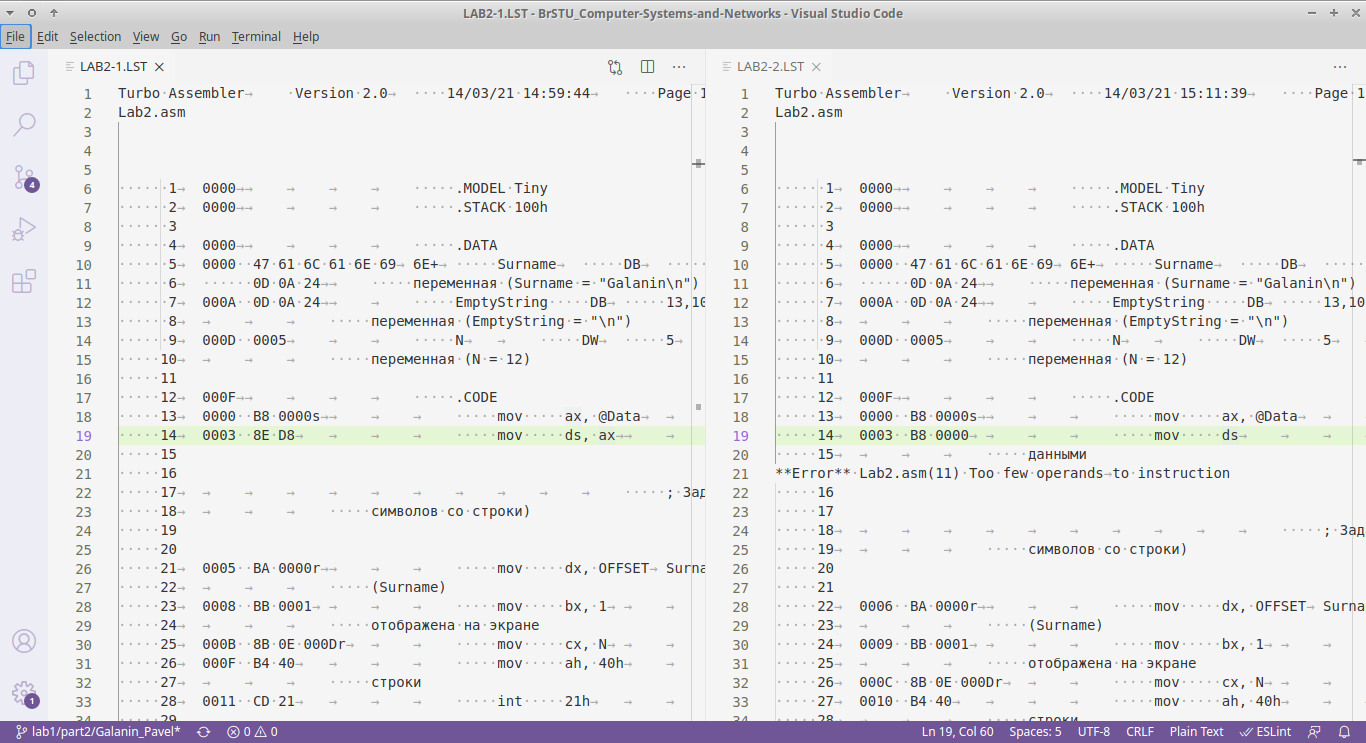
\includegraphics[width=18cm]{../_INCLUDES/lst1-and-lst2.png}
    \caption{Сравнение LAB2-1.LST и LAB2-2.LST в VS Code}
\end{figure}



\subparagraph{Задание 4.5}

\textbf{Условие}:
Восстановить исходную программу и создать загрузочный модуль Lab2.exe (при этом использовать команду \path{d:\tasm\tasm} /zi lab2.asm на этапе трансляции и команду lab2.obj \path{d:\tasm\tlink} /v lab2.obj на этапе компоновки. Привести в отчете назначение ключей /zi и /v).

\textbf{Решение}:

\begin{lstlisting}[language=Terminal]
$ d:\tasm\tasm /zi lab2.asm
\end{lstlisting}

\begin{lstlisting}[language=Out]
Turbo Assembler  Version 2.0  Copyright (c) 1988, 1990 Borland International

Assembling file:   lab2.asm
Error messages:    None
Warning messages:  None
Passes:            1
Remaining memory:  473k
\end{lstlisting}

Размер объектного файла LAB2.OBJ был 309 байт, стал 577 байт (в 1.867 раз больше).

\begin{lstlisting}[language=Terminal]
$ d:\tasm\tlink /v lab2.obj
\end{lstlisting}

\begin{lstlisting}[language=Out]
Turbo Link  Version 2.0  Copyright (c) 1987, 1989 Borland International
\end{lstlisting}

Размер исполняемого файла LAB2.EXE был 597 байт, стал 1,32 КБ (1 360 байт) (в 2.278 раз больше).

Ключ /zi управляет включением в объектный файл номеров строк исходной программы и другой информации, не требуемой при выполнении программы, но используемой отладчиком.

Ключ /v передает в загрузочный файл символьную информацию, позволяющую отладчику TD выводить на экран полный текст исходной программы, включая метки, комментарии и прочее.



\subparagraph{Задание 4.6 (1)}

\textbf{Условие}:
Загрузить программу в отладчик (td \path{d:\asm\lab2}). Какими способами это можно сделать? Отразить способы в отчете.

\textbf{Решение}:



\subparagraph{Задание 4.6 (2)}

\textbf{Условие}:
Выполнить программу по шагам, нажимая клавишу F7, до конца. Проcмотреть содержимое экрана (Alt+F5). После какой операции ассемблера на экране появляются строки?
 
\textbf{Решение}:



\subparagraph{Задание 4.7}

\textbf{Условие}:
Вывести в окне Watch (View->Watch) содержимое выходного буфера. 

\textbf{Решение}:



\subparagraph{Задание 4.8}

\textbf{Условие}:
Выполнить программу (Goto cursor - клавиша F4) до места начала цикла. 

\textbf{Решение}:



\subparagraph{Задание 4.9}

\textbf{Условие}:
Выполнить 2 прохода цикла по F7, контролируя значения регистров. Для этого необходимо открыть окно CPU (View->CPU). Какие регистры изменяются в цикле?

Привести результаты выполнения данного фрагмента программы в отчете в виде таблицы:

\begin{table}[!ht]
   \centering

   \begin{tabular}{|c|c|c|c|c|c|} 
      \hline
      № шага  & IP  & AX  & BX  & CX  & DX  \\ \hline
      \hline
      1       &     &     &     &     &     \\ \hline
      2       &     &     &     &     &     \\ \hline
      ...     &     &     &     &     &     \\ \hline
   \end{tabular}
\end{table}

Объяснить в отчете изменения регистров

\textbf{Решение}:



\subparagraph{Задание 4.10}

\textbf{Условие}:
Остальные проходы цикла выполнить по F8. В чем разница? Привести объяснения в отчете.

\textbf{Решение}:



\subparagraph{Задание 4.12}

\textbf{Условие}: Вывести содержимое выходного буфера в окне Watches. 

\textbf{Решение}:



\subparagraph{Задание 4.13 (1)}

\textbf{Условие}: Вывести содержимое регистра CX буфера в окне Watches в шестнадцатеричном формате (Options->Display options->Hex).

\textbf{Решение}:



\subparagraph{Задание 4.13 (2)}

\textbf{Условие}:
Вывести содержимое регистра CX буфера в окне Watches в десятичном формате (Options->Display options->Decimal).

\textbf{Решение}:



\subparagraph{Задание 4.14}

\textbf{Условие}:
Изменить содержимое регистра CX на величину, меньшую на 2 единицы (Data->Evaluate/Modify->Expression=cx, New Value=cx-2). Выполнить пошагово (F7) программу до конца. Что изменилось? Объяснить в отчете.

\textbf{Решение}:



\subparagraph{Задание 4.15}

\textbf{Условие}:
Выполнить команду Animate из меню Run с задержкой 1000 мс.

\textbf{Решение}:



\subparagraph{Задание 4.16}

\textbf{Условие}:
Сбросить программу по Ctrl-F2. Выполнить первые 2 инструкции. Отменить их действие по Alt-F4. Привести объяснения о результате в отчете.

\textbf{Решение}:



\subparagraph{Задание 4.17 (1)}

\textbf{Условие}:
По шагам пройти до первой после int 21h инструкции. Попытаться по Alt-F4 все отменить. Что получилось? Привести объяснения о результате в отчете.

\textbf{Решение}:



\subparagraph{Задание 4.17 (2)}

\textbf{Условие}:
Сбросить программу по Ctrl-F2. По F7 выполнить первые 6 инструкций. Открыть окно Execution History. Отменить последние 3 шага.

\textbf{Решение}:


